\chapter{Casos de estudio}
\label{cha:CaseStudies}

En este apartado se evaluará el funcionamiento del DSL definido para la creación de un SheetChat. Para ello se tienen que tener en cuenta todas las características previamente mencionadas, la definición del origen de datos, la creación de una conversación que nos proporcione una petición de datos de entrada y su salida asociada; y no menos importante, los recursos que nos permitan humanizar el bot para ofrecer una experiencia de usuario agradable.

Para ello se han elaborado tres ejemplos. El primero de ellos es dado las notas de dos asignaturas impartidas por un profesor, el poder preguntar por las notas de los alumnos. El segundo de los ejemplos permite dado un calendario de sesiones de un congreso científico, en este caso extraido del WISE de 2015\footnote{Calendario con las diferentes sesiones del congreso WISE: \url{http://www4.cis.fiu.edu/wise2015/@schema.html}}, poder obtener información sobre qué sesiones hay en los diferentes slots (u horarios). Por último, el tercer ejemplo permite, dada una hoja de cálculo autogenerada de una búsqueda de restaurantes de Miami en el sitio web Tripadvisor, obtener restaurantes por tipo de comida.

Los tres casos de estudio tendrán la misma estructura. En primer lugar se abordará el problema que el usuario tiene. En segundo lugar se realizará un análisis de las preguntas o cuestiones que tendrá que ser capaz de resolver el chatbot. Posteriormente se hará hincapié en la definición del DSL que tendrá que hacer el usuario. Finalmente se mostrará un ejemplo de interacción entre el chatbot generado y el usuario.

\section{Ejemplo 1: Notas de asignaturas impartidas por un profesor}
\label{sec:EjemploNotas}

Para el primer ejemplo la audiencia objetivo es un profesor de instituto que dispone de las notas de sus alumnos almacenadas en hojas de cálculo. Él es profesor de dos asignaturas Matemática y Física.

\subsection{Hoja de cálculo con los datos}

Para el almacenamiento de las notas de sus alumnos dispone de dos hojas de cálculo, una con las notas de Matemática (ver Figura \ref{fig:SheetNotasMate}) y otra para las calificaciones de la asignatura de Física (ver Figura \ref{fig:SheetNotasFisica}).

Tal y como se puede observar en la Figura \ref{fig:SheetNotasMate} el profesor tiene las notas de cada uno de sus alumnos que va rellenando a medida que se les evalúa de los diferentes aspectos de las asignaturas. Por lo tanto, cada fila representa a un alumno y cada columna a cada concepto a evaluar de la asignatura.

En el método de evaluación empleado por el profesorado se tiene en cuenta trabajos de clase o ejercicios y exámenes durante la evaluación continua. En caso de que la media ponderada de estos parciales supere un 5 el alumno habrá aprobado mediante la evaluación continua. En caso contrario, tendrá que presentarse a un examen final con todo el temario del curso. A modo de ejemplo se puede visualizar en la Figura \ref{fig:SheetNotasMate} como el alumno Adrian Arana ha aprobado la evaluación continua con un 5.9 mientras que Alberto Ballester tuvo que presentarse al examen final para aprobar dado que en la evaluación continua su nota era de 3.85.

\begin{figure}[htb]
	\centering
	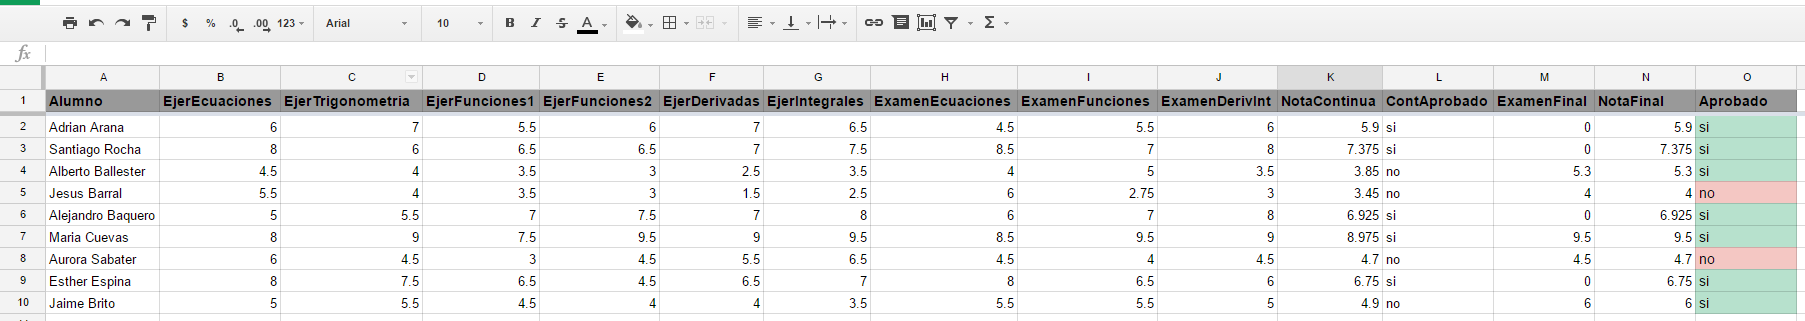
\includegraphics[width=0.8\textwidth]{./figs/sheetNotasMate.png}
	\caption{Hoja de cálculo del profesor para la asignatura de matemática.} \label{fig:SheetNotasMate}
\end{figure}

\begin{figure}[htb]
	\centering
	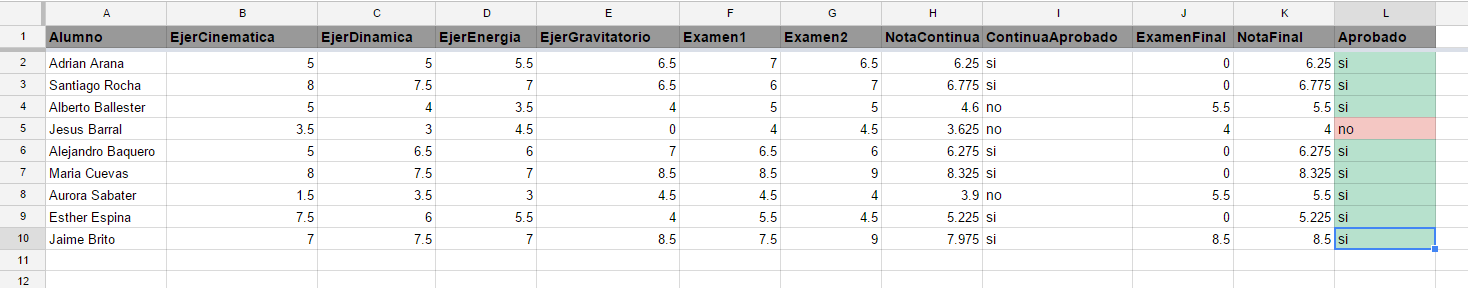
\includegraphics[width=0.8\textwidth]{./figs/sheetNotasFisica.png}
	\caption{Hoja de cálculo del profesor para la asignatura de física.} \label{fig:SheetNotasFisica}
\end{figure}

\subsection{Análisis de preguntas}
\label{sec:queriesNotas}

Una vez conocidos los datos almacenados, el profesor que quiere generar un chatbot tiene que tener en cuenta qué tipo de análisis quiere hacer sobre los datos, o dicho de otra manera, qué consultas va a realizar sobre los datos. Debería de ser capaz de decidir cuales son las preguntas más habituales sobre esos datos o las que más frecuentemente le piden sus alumnos. Dado que son asignaturas diferentes y su método de evaluación no es exactamente el mismo, las preguntas que se puede llegar a realizar también son diferentes.

A continuación se recogen algunas de las preguntas que podría hacer el profesor:
\begin{itemize}
	\item \textbf{¿Cuál es la nota que tiene un alumno en cada uno de los ejercicios de mate/fisica?} Es habitual preguntar por la nota en uno de los ejercicios o en el conjunto de los mismos a lo largo de la evaluación.
	\item \textbf{¿Cuál es la nota de un alumno en los exámenes parciales de mate/física?} Al igual que sucede con los ejercicios, es interesante conocer las notas de los exámenes parciales.
	\item \textbf{¿Se debe de presentar un alumno al examen final de mate?} O dicho de otra manera, ¿ha aprobado la evaluación continua?
	\item \textbf{¿Qué nota debe de sacar un alumno en los exámenes de física para aprobar la asignatura?} O preguntado de otra manera, ¿Qué nota ponderada tiene en los ejercicios de evaluación continua?
	\item \textbf{¿Ha aprobado un alumno la asignatura de física?} De esta manera se sabe si un alumno ha de presentarse a la segunda convocatoria de física o no.
\end{itemize}

\subsection{Definición del DSL}

Como se ha comentado en el Capítulo \ref{cha:AnalysisAndDesign} hay que definir mediante el uso del DSL de SheetChat el origen de los datos y los intents para cada una de las consultas que se quiera extraer de la hoja de cálculo previamente definidas en el Apartado \ref{sec:queriesNotas}.

Si se observa la Figura \ref{fig:DSLNotas} se puede observar cómo es la definición de las hojas de cálculo a consultar. De igual manera se define una descripción para el chatbot y un mensaje de bienvenida que nos ayude a recordar alguna de las funcionalidades del bot. Posteriormente se muestra un intent de los que deberá de definir el profesor que vaya a utilizar el chatbot.

El intent a resolver es el de obtener la nota de los ejercicios de mate de un determinado alumno. El origen de datos por tanto será la hoja de NotasMate. Se define que las columnas que el bot debe de responder son las de los ejercicios. También se define que sólo se desea un resultado, ya que sólo se pregunta por un alumno concreto. Esta característica es útil para mostrar un número determinado de resultados. En este caso cada alumno se identifica inequívocamente por el nombre y apellido. También se indica que se muestre el nombre de la columna (en este caso el nombre del ejercicio).

Dentro del intent también se definen las entidades de filtrado. En este caso se define la columna Alumno. El tipo de filtrado utilizado es LIKE, que tiene la misma funcionalidad que el like de SQL. Esto permite no tener que introducir nombre y apellido del alumno, si no introducir parcialmente su nombre a la hora de filtrar. En lugar de exigir al usuario escribir Adrian Arana, podrá preguntar por las notas de Adrian o de Arana. Por último se definen mensajes que permitan al usuario preguntar de una manera más amigable (o humana, ver Apartado \ref{sec:Humanization}) por las entidades que hacen falta.

\begin{figure}[htb]
	\centering
	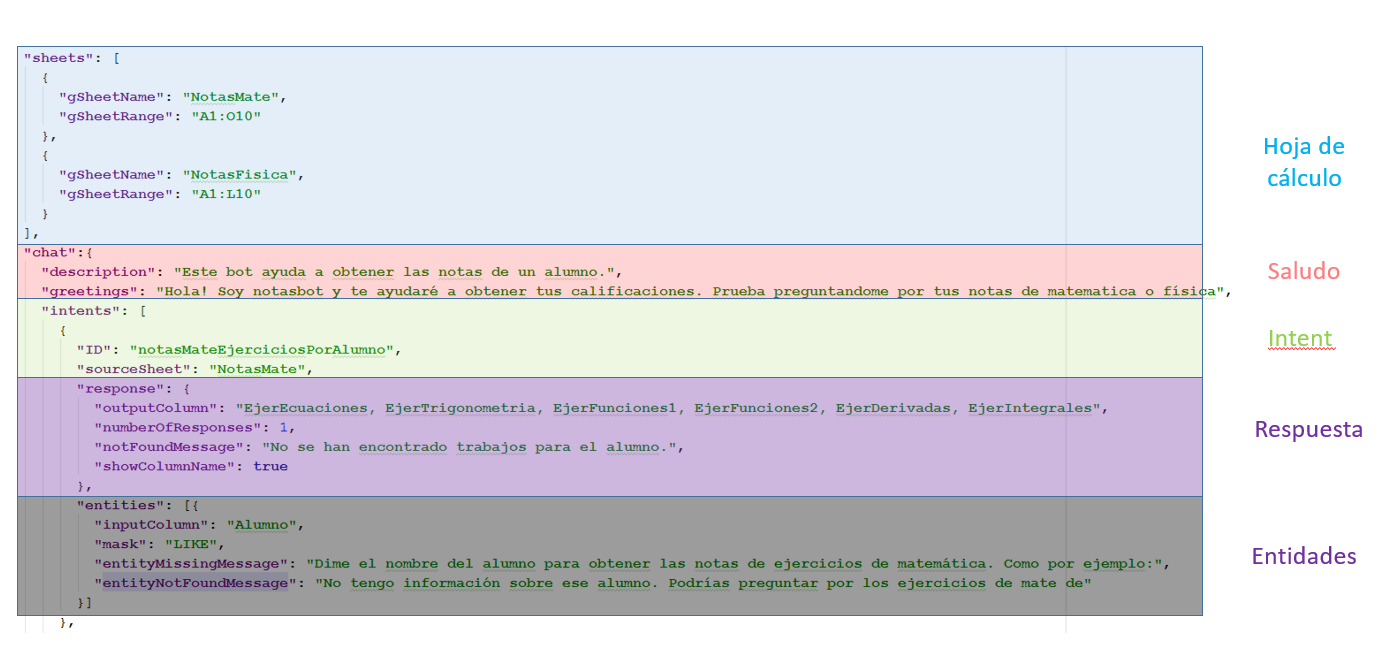
\includegraphics[width=1.2\textwidth]{./figs/DSLNotas.png}
	\caption{DSL con la definición de las Sheet y un intent a utilizar en el ejemplo de notas.}
	\label{fig:DSLNotas}
\end{figure}

Algunas preguntas son más difíciles de formular debido a la naturaleza de los datos. Sin embargo, SheetChat ofrece algunos mecanismos que permiten resolver funciones matemáticas a la hora de realizar consultas sobre los datos. Se puede observar en la pregunta relacionada con obtener la nota ponderada. La nota ponderada de los ejercicios de Física el profesor lo tiene definido de una manera determinada. Esto no es una columna como tal dentro de la hoja de cálculo, si no que es una entidad derivada. En la Figura \ref{fig:DSLNotasPonderada} se observa que dentro del response hay una expresión matemática que define qué es la nota ponderada de los ejercicios. De igual manera, en las respuestas se puede proporcionar un mensaje personalizado para mejorar la humanización del bot ofreciendo una respuesta más sencilla de interpretar por un humano.

\begin{figure}[htb]
	\centering
	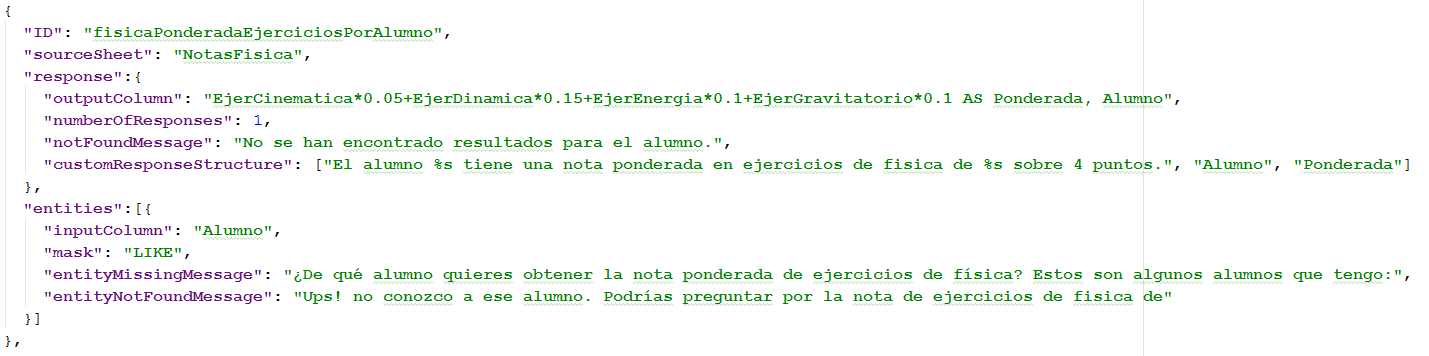
\includegraphics[width=0.8\textwidth]{./figs/DSLNotasPonderada.png}
	\caption{Definición de la pregunta para obtener la nota ponderada de los ejercicios de física del ejemplo de notas.}
	\label{fig:DSLNotasPonderada}
\end{figure}

\subsection{Ejemplo de uso del chatbot}

A continuación se puede visualizar cómo sería un ejemplo de interacción entre un ser humano y el bot que se ha generado a partir del DSL de SheetChat en el ejemplo de las notas. En la Figura \ref{fig:EjecucionNotas1} se puede observar un intercambio de mensajes para obtener información respecto al alumno Alberto. En primer lugar se ha saludado al chatbot para que este proporcione su mensaje de bienvenida. Esta interacción no es necesaria si se conocen cuales son las características del chatbot. Posteriormente se le han preguntado por los resultados de alberto en matemática: si habia aprobado la evaluación continua y las notas que ha obtenido para conocer la causa de su suspenso. De igual manera se han realizado dos preguntas respecto a las notas de física.

\begin{figure}[htb]
	\centering
	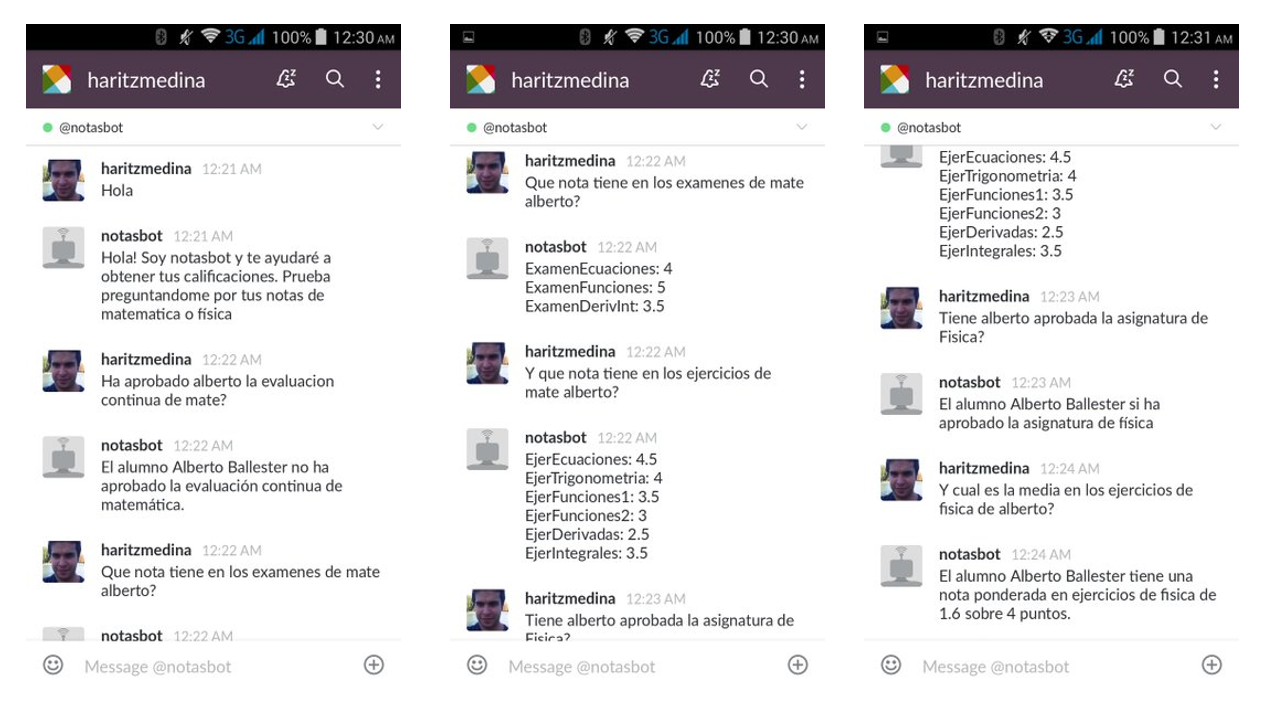
\includegraphics[width=0.8\textwidth]{./figs/ejecucionNotas1.png}
	\caption{Interacciones del usuario a la hora de consultar las notas de Alberto.}
	\label{fig:EjecucionNotas1}
\end{figure}

En este caso el chatbot ha inferido cuales eran los intents del usuario y a su vez la entidad necesaria para cada una de ellas, en este caso el nombre del alumno. Si se obtienen de la frase de manera adecuada los intents y las entidades el chatbot proporciona la respuesta. En caso de que se haya inferido el intent pero no las entidades, preguntará por ellas (ofreciendo sugerencias que ayuden al usuario). Esto sucede en la Figura \ref{fig:EjecucionNotas2} dado que no se le había proporcionado ningún nombre a la hora de preguntar por la media en los ejercicios de física. De igual manera, si se le proporciona un nombre no existente, el chatbot le seguirá ofreciendo sugerencias.

\begin{figure}[htb]
	\centering
	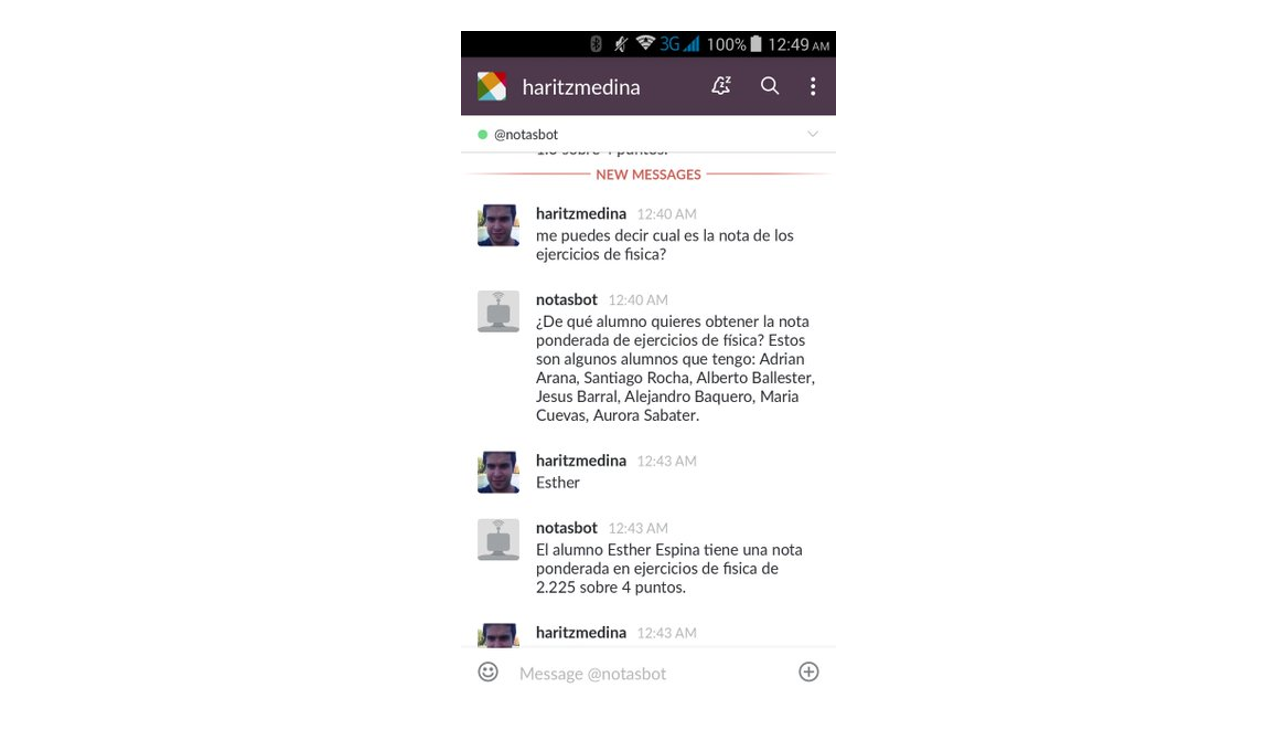
\includegraphics[width=0.8\textwidth]{./figs/ejecucionNotas2.png}
	\caption{El chatbot recomienda algunos nombres en caso de que no se defina o se defina un nombre inexistente para hacer el filtrado en la hoja de cálculo.}
	\label{fig:EjecucionNotas2}
\end{figure}

\section{Ejemplo 2: Calendario de sesiones en un congreso científico}

Los congresos disponen de un calendario complejo, dónde hay trabajos más o menos interesantes o relevantes con la rama de especialización que tiene el asistente. Es por ello que acudir a las sesiones más afines a tu trabajo es importante. Es interesante disponer de información in situ de cuales son las próximas charlas que habrá, dónde o quién las presenta. Sin embargo, los sitios webs rara vez están preparados para su navegación por el móvil o se pierde mucho tiempo en encontrar los eventos a los que se desea acudir. Es una información relevante y que se desea conocer en el momento.

Este ejemplo se centra en ofrecer una alternativa en forma de bot mediante una hoja de cálculo creada a partir del horario de la conferencia WISE 2015 \footnote{Programa del WISE 2015 (Web Information System Engineering) \url{http://www4.cis.fiu.edu/wise2015/@schema.html}}.

\subsection{Hoja de cálculo con los datos}

Como se ha mencionado previamente la hoja de cálculo es creada a partir de una tabla con el programa disponible en el sitio web. En la Figura \ref{fig:SheetConference} se puede observar el calendario de las diferentes sesiones que están presentes en el congreso. Cada sesión tiene asociada un día y un slot (una franja horaria) donde se exponen trabajos. En algunos de los slots se produce un solapamiento de múltiples sesiones, por lo que es interesante que el usuario conozca cuales son las charlas para elegir la más interesante.

\begin{figure}[htb]
	\centering
	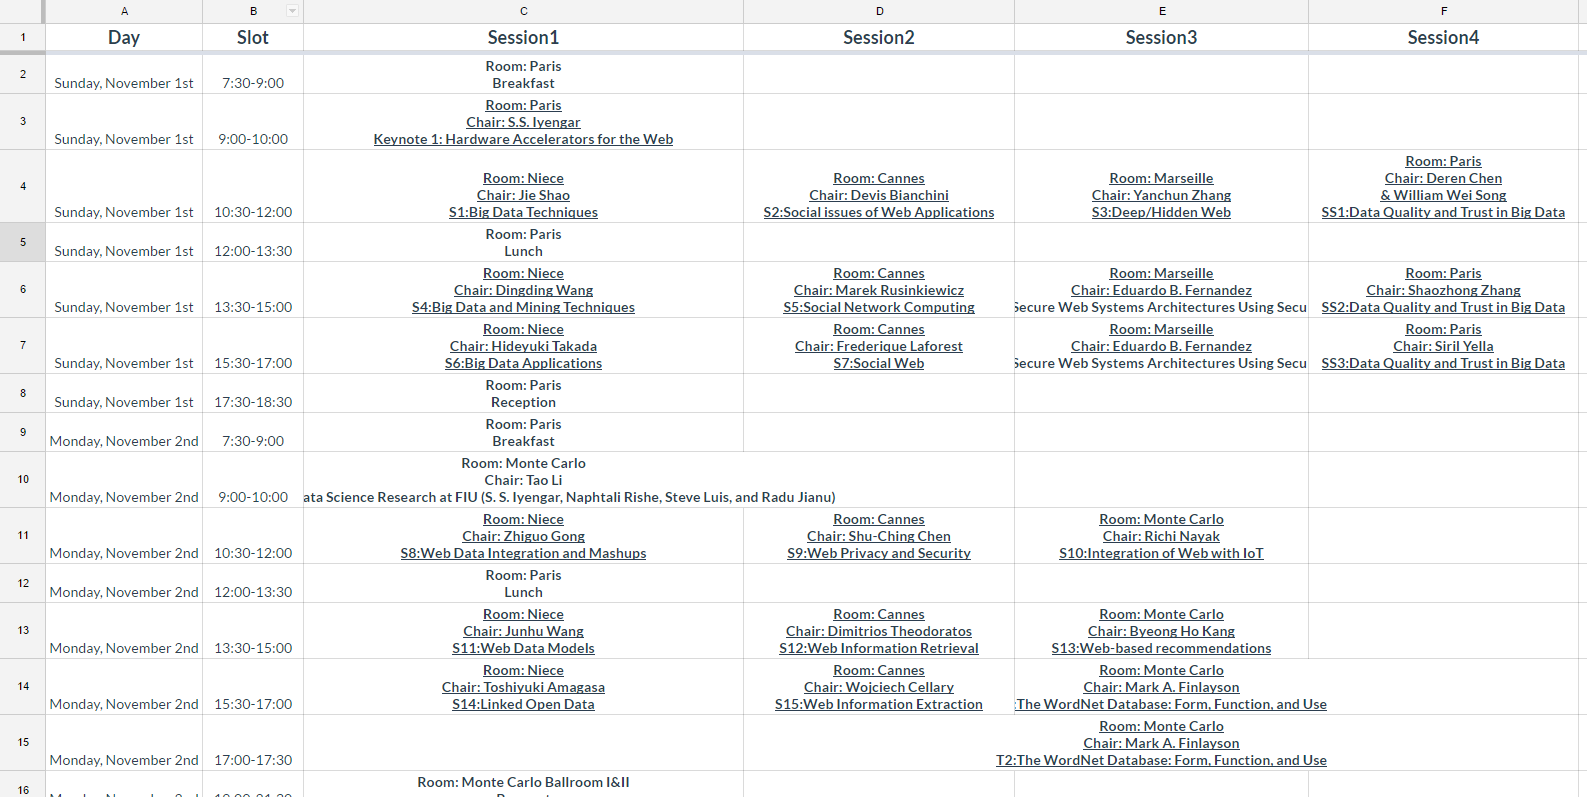
\includegraphics[width=0.8\textwidth]{./figs/sheetConference.png}
	\caption{Hoja de cálculo con el programa del WISE 2015.}
	\label{fig:SheetConference}
\end{figure}

\subsection{Análisis de preguntas}

Como se ha comentado previamente, el usuario del bot tiene como objetivo poder conocer el programa del congreso durante la estancia en él. Algunas de las preguntas que le pueden surgir durante el evento están recogidas a continuación:
\begin{itemize}
	\item \textbf{¿Cuáles son las charlas en un horario concreto, es decir, qué eventos hay en esa franja horaria?} De los eventos que existan en esa franja horaria, el asistente al congreso podría decantarse por la que más interesante le resulte.
	\item \textbf{¿Qué eventos hay relacionados con un tema (o topic) en particular?} De esta manera el usuario sabrá con una simple pregunta en qué horarios están programadas charlas interesantes para él.
	\item \textbf{¿Quiero conocer en qué sesiones participa una persona?} Los investigadores conocen el trabajo de algunas personas y puede interesarle saber si estas personas participan como expertas en la materia de una determinada sesión.
\end{itemize}

\subsection{Definicion del DSL}

El diseño del chatbot en este ejemplo constará de una única hoja de cálculo y de dos intents. A pesar de que previamente se han definido 3 cuestiones, sólo hace falta definir dos intents debido a que la obtención de las sesiones relacionadas con un tema en concreto o presidido por un chairman concreto se pueden unir en una. Esto es debido a la naturaleza de los datos. Una columna sesión tiene como valor un string que incluye ambas informaciones. A la hora de realizar el filtrado, se filtra por valor de la columna que se desee. Visto en un ejemplo, observando la sesión 1 del domingo en el slot 10:30-12:00, es lo mismo filtrar por el topic \emph{Hardware Accelerators for the Web} por la habitación \emph{Paris} o el chairman \emph{Iyengar}, se obtendrá como resultado el dia y slot de esa sesión.

Por otro lado, en este ejemplo, surge la novedad de filtrar por más de una columna. En la Figura \ref{fig:DSLConference} se observa remarcado en color azul el entity definido. En este caso se han definido cuatro columnas que actuarán como filtro. A la hora de preguntar por el topic o chairman, el chatbot buscará si se dan positivos en cualquiera de las cuatro columnas. En caso de que el valor introducido por el usuario dé positivo por alguna de las cuatro columnas, se le mostrará el día y la hora (o slot) de ese evento.

\begin{figure}[htb]
	\centering
	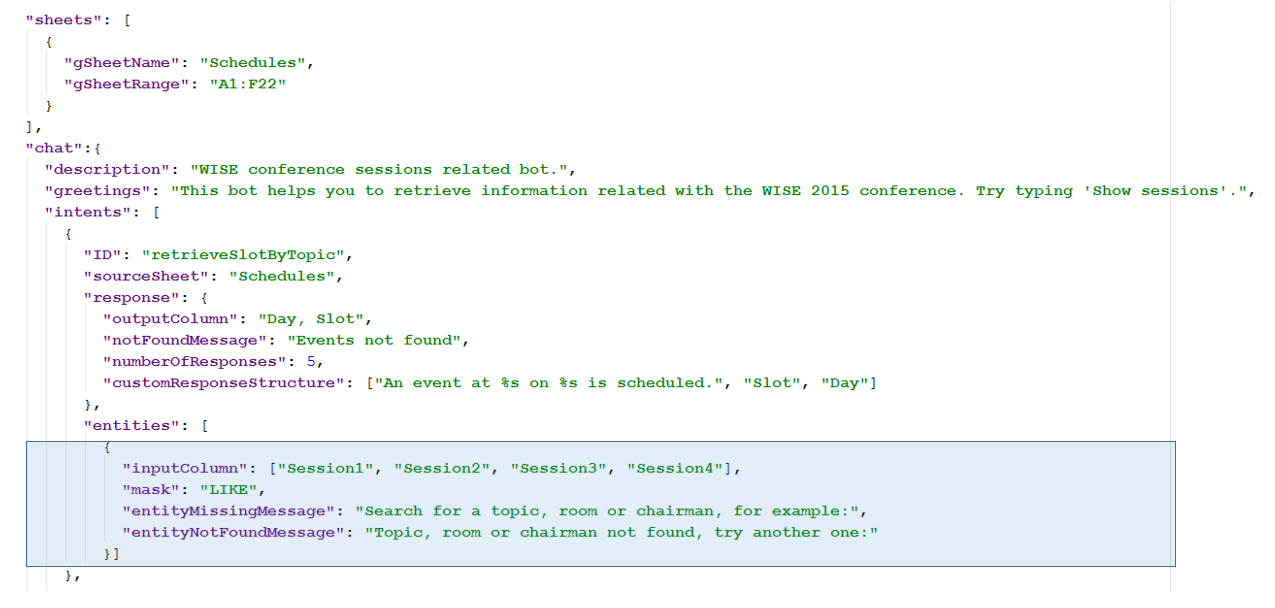
\includegraphics[width=0.8\textwidth]{./figs/DSLConference.png}
	\caption{Implementación del chatbot de la conferencia. Cabe destacar remarcado en azul el intent con input multicolumna.}
	\label{fig:DSLConference}
\end{figure}

\subsection{Ejemplo de uso del chatbot}

A continuación se presenta un ejemplo de interacción real con el chatbot desarrollado para el programa de las conferencias. Para la obtención de las sesiones en una franja horaria concreta, tal y como se ha mencionado en la implementación del chatbot, se requiere de dos parámetros (el día y el slot). En la Figura \ref{fig:EjecucionConference} el Chatbot guía al usuario mediante preguntas para obtener la información suficiente de a qué slot se refiere el usuario. En este caso realiza una pregunta respecto a los días y otra respecto al slot. Si el usuario hubiese añadido esa información a la hora de hacer la pregunta, el chatbot podría haber inferido estas entidades y ahorrarse los pasos de preguntarlo. Esto es lo que sucede en la pregunta de la imagen derecha, donde el usuario ha proporcionado un criterio de búsqueda.

\begin{figure}[htb]
	\centering
	\includegraphics[width=0.8\textwidth]{./figs/EjecucionConferencia.png}
	\caption{Interacción del usuario a la hora de preguntar por los eventos en una hora concreta (Imagen izquierda y central) y consulta respecto a un topic concreto (Imagen derecha).}
	\label{fig:EjecucionConference}
\end{figure}


\section{Ejemplo 3: Búsqueda de restaurantes de Tripadvisor}

En este tercer caso de estudio se muestra además de un nuevo contexto de uso, el uso de un origen de datos web. En la actualidad la mayoría de información se puede recabar en la red, sin embargo esta no suele tener una estructura utilizada en un ámbito general como son las tablas de bases de datos o las hojas de cálculo.

En este ejemplo se mostrará cómo se pueden realizar búsquedas en restaurantes extraídos del sitio web Tripadvisor. Tripadvisor es un sitio web de opinión sobre hoteles, restaurantes, y otros lugares de ocio. En su web se pueden filtrar los resultados en base a localización (como una ciudad o provincia), características del sitio (número de estrellas de un hotel o tipo de comida de un restaurante) y otros muchos aspectos. Concretamente en este ejemplo se ha realizado una búsqueda de restaurantes en Miami (Estados Unidos), que es lo que se puede observar en la Figura \ref{fig:TripadvisorMiami}.

\begin{figure}[htb]
	\centering
	\includegraphics[width=0.8\textwidth]{./figs/tripadvisorMiami.png}
	\caption{Búsqueda de restaurantes de Miami en Tripadvisor}
	\label{fig:TripadvisorMiami}
\end{figure}

La idea para este ejemplo es demostrar que estos datos en la web pueden ser extraidos a una hoja de cálculo y generar un chatbot mediante la herramienta SheetChat.

\subsection{Hoja de cálculo con los datos}

Como se ha mencionado al comiendo de este caso de estudio, el objetivo es poder representar estos datos en forma de hoja de cálculo. Para ello en la web existen múltiples herramientas de web scraping (extracción de información de la web). A pesar de que la web de tripadvisor muestre los restaurantes en un formato más amigable para el ser humano, si que todos los restaurantes comparten una estructura similar. En la Figura \ref{fig:TripadvisorMiami} se observa que todos los restaurantes tienen un hyperlink con el nombre del restaurante donde pinchando saldría la ficha del restaurante en cuestión. Cada restaurante tiene una imagen asociada, un número de opiniones, dos breves opiniones, el precio promedio del menú del restaurante y el tipo de comida. Precisamente, el encontrar patrones y extraer datos es el objetivo de herramientas como Import.io\footnote{\href{https://www.import.io/}{Import.io} extracción de datos tabulares a partir de sitios web.}.

El funcionamiento de import.io permite extraer una tabla con los resultados de la búsqueda de restaurantes de Miami. En el Anexo \ref{anx:importio} se puede profundizar en el funcionamiento de la herramienta. Para el ejemplo, simplemente la hoja de cálculo que obtenemos es la presentada en la Figura \ref{fig:SheetTripadvisor}. Mediante import.io se han extraido 400 restaurantes en Miami. En la tabla se pueden observar las columnas sobre las que podremos realizar preguntas posteriormente al bot, nombre del restaurante (Name), sitio web con la ficha de Tripadvisor (url), rango de precios de los menús (RangePrice) o tipo de comida (Cuisines).

\begin{figure}[htb]
	\centering
	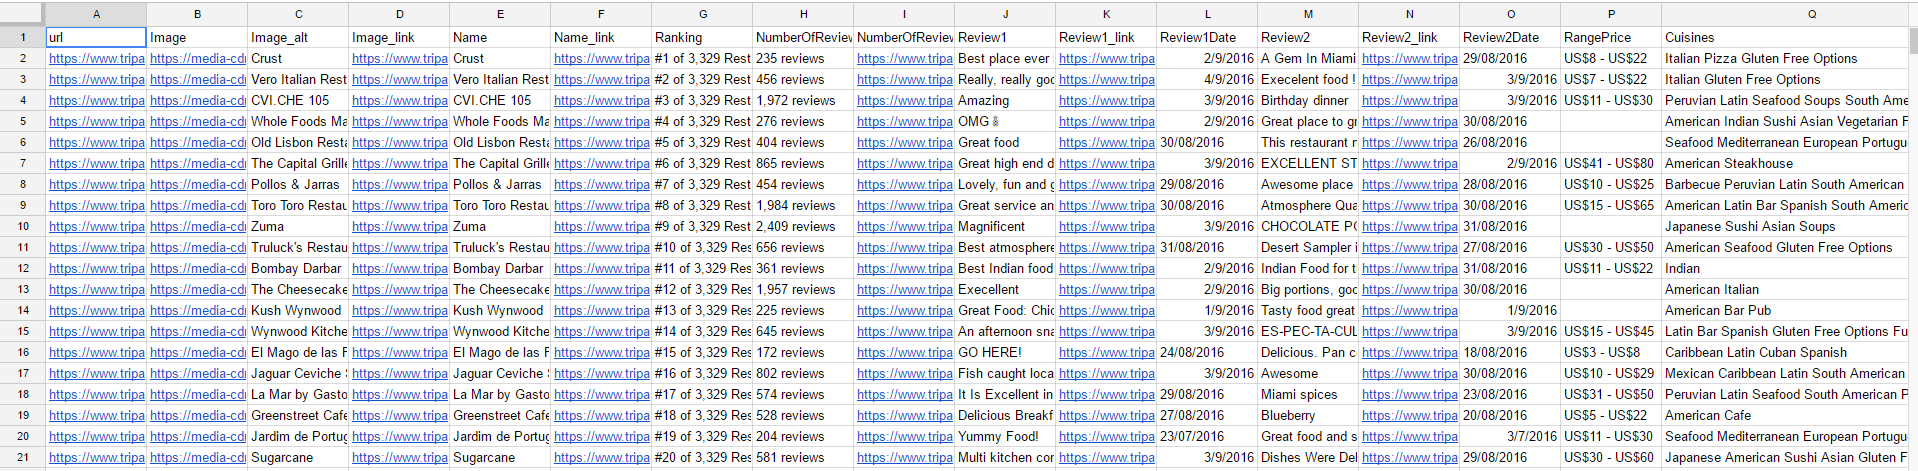
\includegraphics[width=0.8\textwidth]{./figs/sheetTripadvisor.png}
	\caption{Hoja de cálculo con restaurantes de Miami extraidos de Tripadvisor.}
	\label{fig:SheetTripadvisor}
\end{figure}

\subsection{Análisis de preguntas}

Tras observar los datos extraídos de Tripadvisor, el usuario podría hacer diferentes preguntas. En este caso se ha decidido que pueden ser interesantes las que se presentan a continuación:
\begin{itemize}
	\item \textbf{¿Me podrías ayudar a buscar restaurantes con comida italiana?} Al igual que se puede preguntar por italiana, se puede preguntar por cualquier tipo de comida que se haya extraído de los restaurantes situados en Miami.
	\item \textbf{¿Qué restaurantes vegetarianos hay por menos de 45 dolares?} Similar a la pregunta anterior, con la condición de precio máximo, ya que son dos aspectos que se suelen mirar frecuentemente a la hora de buscar un restaurante, si gusta la comida y el precio.
	\item \textbf{¿Qué opinión hay sobre un restaurante concreto?} Mediante la opinión de otros usuarios extraída del sitio web, el usuario del Chatbot puede deducir si un restaurante es bueno o no.
\end{itemize}

\subsection{Definicion del DSL}
\label{sec:DSLTripadvisor}

Para este ejemplo se trabajará la definición de las interacciones para las dos primeras cuestiones previamente definidas. En la Figura \ref{fig:DSLTripadvisor1} se ve la definición para la primera de las preguntas, dónde la entidad de entrada es la columna \emph{Cuisines} (tipo de cocina) y en la salida se mostrará un mensaje personalizado con el nombre, el tipo de comida, el rango de precio y un link para abrir la ficha en Tripadvisor.

Se ha observado que el resultado que ofrece el chatbot (junto con la previsualización de links de la plataforma Slack) hace que el chatbot al ofrecer la respuesta sea muy verboso. Por esa razón, se ha decidido que se limite a tres el número de respuestas máximas que va a recibir el usuario.

\begin{figure}[htb]
	\centering
	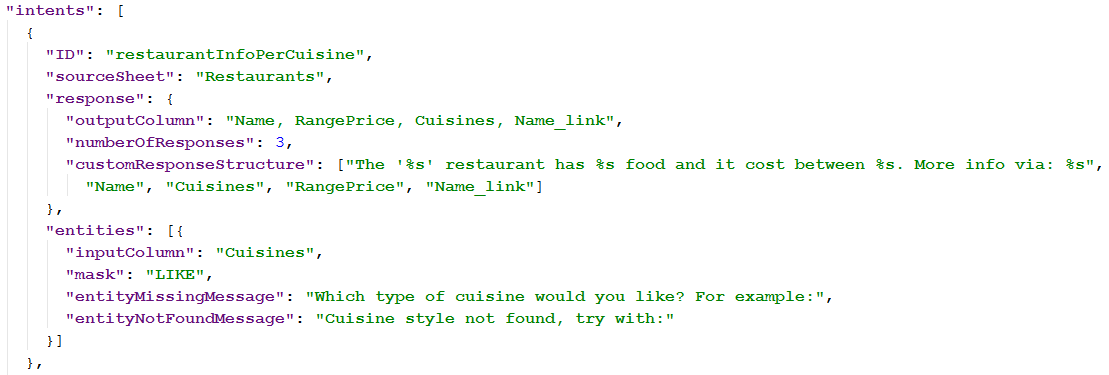
\includegraphics[width=0.8\textwidth]{./figs/DSLTripadvisor1.png}
	\caption{DSL de SheetChat que describe el intent para la búsqueda por tipo de comida de los restaurantes de Tripadvisor.}
	\label{fig:DSLTripadvisor1}
\end{figure}


De igual manera, en la Figura \ref{fig:DSLTripadvisor2} se muestra la definición utilizando el DSL de SheetChat donde el usuario hará peticiones respecto a un precio máximo y un tipo de comida concretos, es decir, hay dos entidades participantes a la hora de realizar el filtrado entre los 400 restaurantes. Como novedad cabe destacar que el valor del campo Mask en lugar de ser LIKE (que sirve para comparar strings), se utiliza el símbolo < para designar que es un valor númerico y que el filtro rechazará los resultados mayores que el precio máximo delimitado por el usuario a la hora de interaccionar con el Chatbot, tal y cómo se muestra en el Apartado \ref{sec:EjemploUsoTripadvisor}.

\begin{figure}[htb]
	\centering
	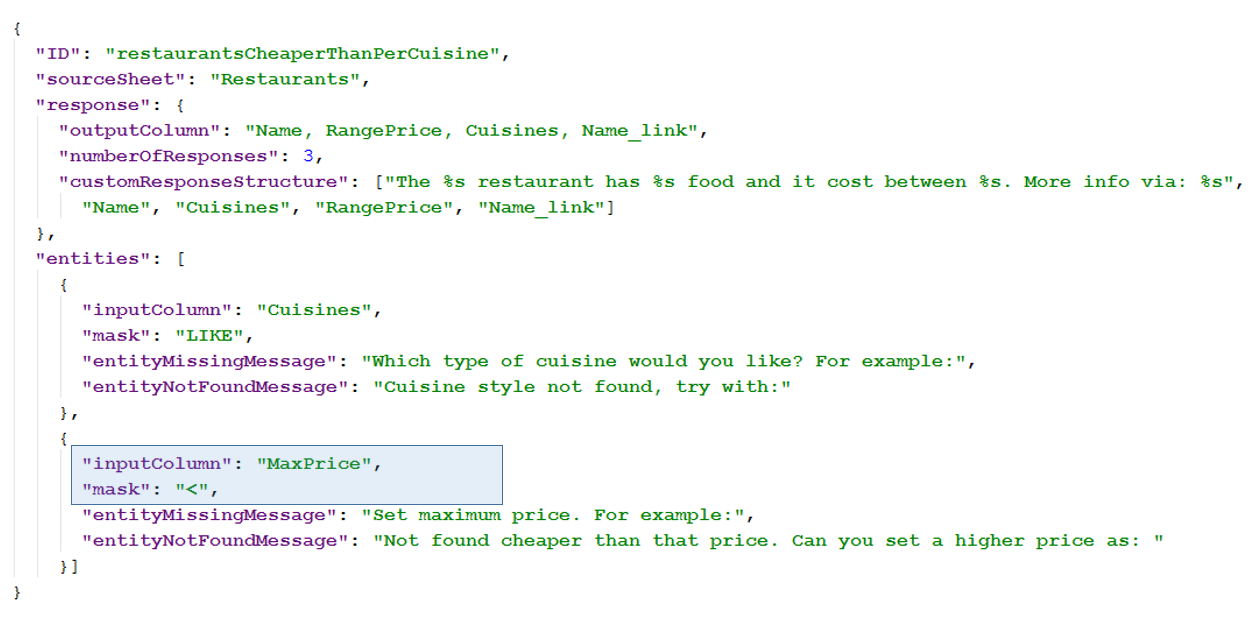
\includegraphics[width=0.8\textwidth]{./figs/DSLTripadvisor2.png}
	\caption{DSL de SheetChat que describe el intent para la búsqueda por precio máximo (resaltado en azul) y tipo de comida de los restaurantes de Tripadvisor.}
	\label{fig:DSLTripadvisor2}
\end{figure}

\subsection{Ejemplo de uso del chatbot}
\label{sec:EjemploUsoTripadvisor}

Tras el diseño del Chatbot mediante el DSL de SheetChat a continuación se presenta cómo sería la experiencia de uso de este chatbot por parte de un usuario.

En la Figura \ref{fig:EjecucionTripadvisor1} el usuario en primer lugar saluda al Chatbot y este le ofrece alguna de sus funcionalidades por si acaso el usuario no se acuerda de qué trata este chatbot o qué funcionalidades tenía. Posteriormente se dispone a preguntar por restaurantes italianos. El chatbot le responde con tres resultados, el número máximo de resultados que se indicó en el diseño del chatbot (ver Apartado \ref{sec:DSLTripadvisor}).

\begin{figure}[htb]
	\centering
	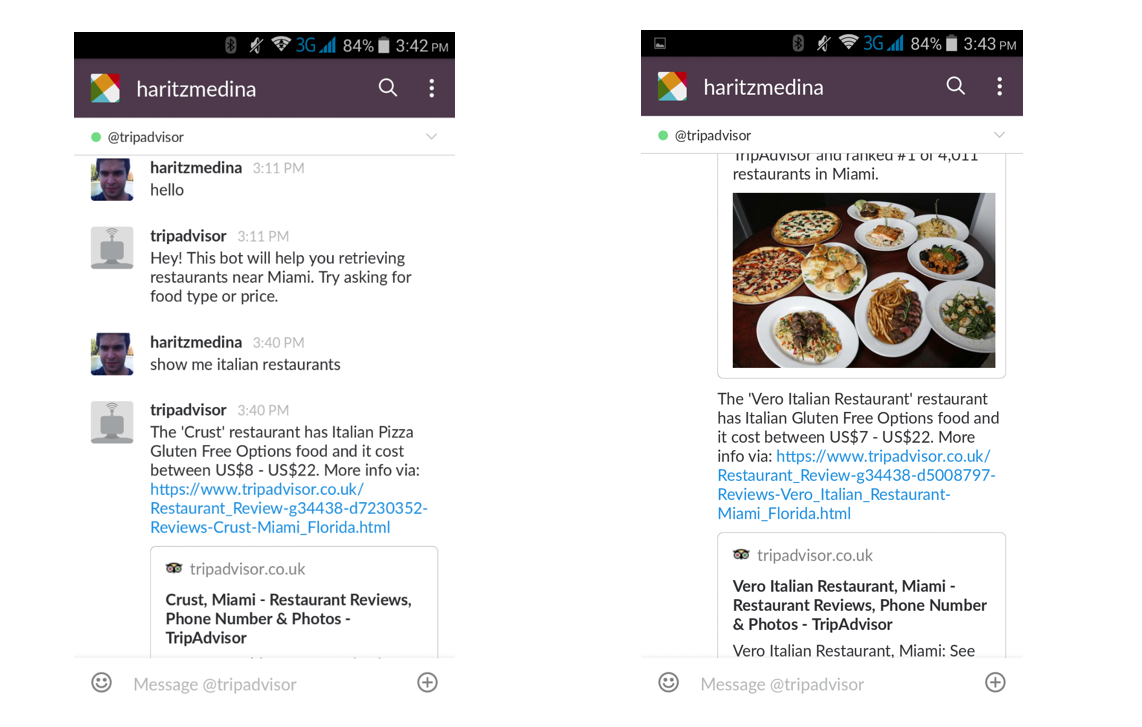
\includegraphics[width=0.8\textwidth]{./figs/ejecucionTripadvisor1.png}
	\caption{Interacción entre el usuario y el chatbot que recomienda restaurantes en base a un tipo de cocina.}
	\label{fig:EjecucionTripadvisor1}
\end{figure}

En la interacción de la Figura \ref{fig:EjecucionTripadvisor2} se observa que al usuario las recomendaciones de los restaurantes italianos le ha resultado cara. Por lo tanto decide preguntar por restaurantes con precio menor a 15 dolares. El chatbot ha detectado que el usuario está preguntando por restaurantes con un precio máximo y un tipo de cocina determinado. El chatbot restringe las respuestas en base a ese nuevo filtro y muestra el único restaurante que cumple esas características. En caso de que no hubiese ningún restaurante que cumpliese ambos criterios preguntaría por las entidades nuevamente.

\begin{figure}[htb]
	\centering
	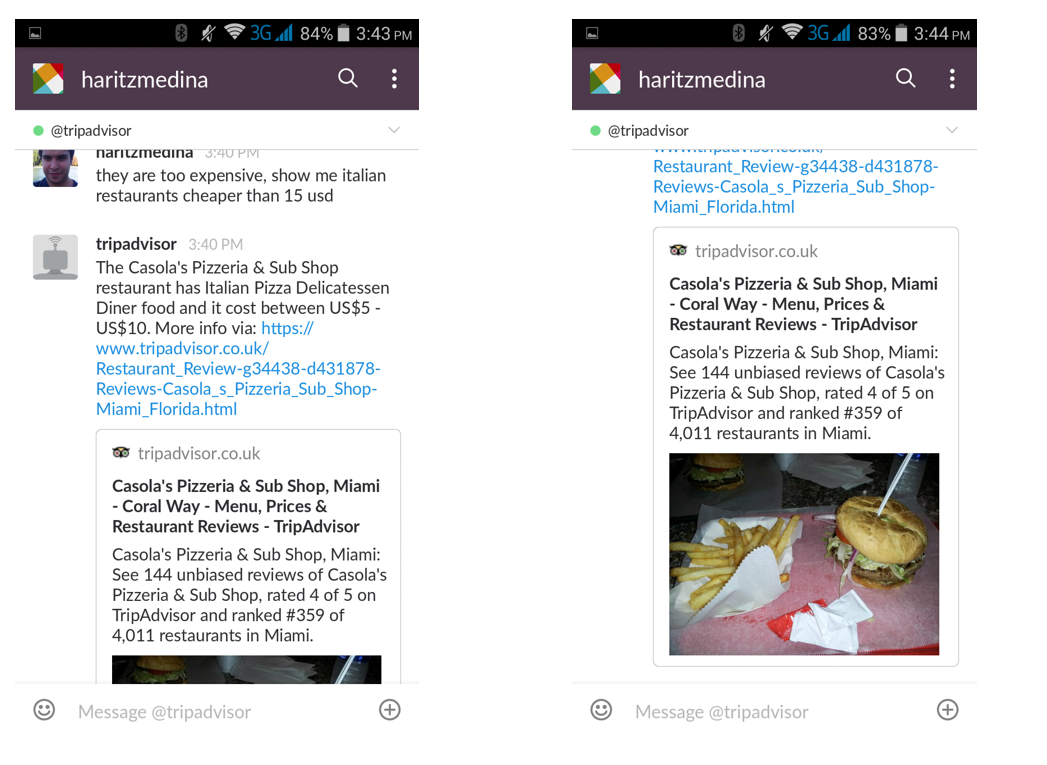
\includegraphics[width=0.8\textwidth]{./figs/ejecucionTripadvisor2.png}
	\caption{El bot de Tripadvisor recomienda restaurantes italianos con precio menor a 15 dolares por petición del usuario.}
	\label{fig:EjecucionTripadvisor2}
\end{figure}

De esta manera, mediante el uso de un chatbot, el usuario evita tener que aplicar filtros en el sitio web de Tripadvisor que en una configuración móvil suele resultar en lineas generales bastante farragoso.